\documentclass[11pt]{article}
\usepackage{amsmath,textcomp,amssymb,geometry,graphicx,enumerate}
\usepackage[linesnumbered,ruled,vlined]{algorithm2e}
\raggedbottom
\usepackage{placeins}

% Allow more floats per page and reduce empty space
\renewcommand{\topfraction}{0.9}
\renewcommand{\bottomfraction}{0.9}
\renewcommand{\textfraction}{0.1}
\renewcommand{\floatpagefraction}{0.7}
\setcounter{totalnumber}{6}
\setcounter{topnumber}{4}
\setcounter{bottomnumber}{4}
\usepackage{hyperref}
\usepackage{subcaption}
\usepackage{float}
\usepackage{booktabs}
\usepackage{multirow}
\usepackage{xcolor}
\usepackage{colortbl}
\def\Homework{$3$} % Number of Homework
\def\Session{Spring 2026}

\title{CS536 --- Spring 2026 --- TCP Expo}
\author{Group: Youngjun Yoo, Dylan Boyer, Alejandro Griffith, Douglas Muir, Amit Manchella}
\markboth{CS536 --- \Session\  TCP Expo}
\date{}

\newenvironment{qparts}{\begin{enumerate}[{(}a{)}]}{\end{enumerate}}

\textheight=9in
\textwidth=6.5in
\topmargin=-.75in
\oddsidemargin=0.25in
\evensidemargin=0.25in

\hypersetup{
    colorlinks=true,
    linkcolor=blue,
    filecolor=blue,
    urlcolor=blue,
}


\begin{document}
\maketitle
\section{TCP Expo Overview}
\subsection*{Relevant Links}
\href{https://github.com/CS536-Group2026/hw2/tree/main}{HW 2 Repo Link} \\
\href{https://github.com/CS536-Group2026/hw3/tree/main}{HW 3 Repo Link} \\ \\
\href{https://github.com/CS536-Group2026/hw3/blob/main/readme.md#kernel-module-setup}{**INSTRUCTIONS ON HOW TO SET UP OUR KERNEL MODULE**}

\subsection*{Strategy}
TCP Expo is a delay-based congestion control algorithm we built as a kernel module for CS536. Instead of waiting for packet loss to know the network is congested (like Reno and CUBIC do), Expo watches the round-trip time. When RTT starts climbing, it means packets are sitting in router queues — the network is getting full even though nothing has been dropped yet.
\\ \\
The core idea is momentum: we track how much RTT has inflated compared to the baseline (the lowest RTT we've seen). If RTT is still close to baseline, we grow the window aggressively. If it's spiking up, we slow down. If it spikes past 75\% inflation, we do a small reduction called a Negative Pulse (thanks to the professor advice) — dropping the window by about 3\% to reduce the queue back down without throwing away throughput.
\\ \\
There are three zones:
\begin{itemize}
    \item Clean zone ($<$ 30\% RTT inflation) — grow fast, the pipe has room
    \item Build zone (30–75\%) — some queuing, grow carefully
    \item Expo zone ($>$ 75\%) — too much delay, fire a Negative Pulse
\end{itemize}
This lets Expo fill the pipe without flooding it. Furthermore, in the clean zone we have an acceleration system: the longer the connection goes without hitting congestion, the faster we let the window grow (up to 16x the base rate). We also wanted to have fun with it and experimented a bit—we start with an initial window of 20 segments instead of the default 10, which gets data moving faster on high-bandwidth links.
\\ \\
If you want more information on how our algorithm works, \href{https://github.com/CS536-Group2026/hw3/blob/main/explanation.md}{click here.}

\newpage
\section{Testing with suite from HW 2}

\newpage
\section{Extended Testing and Analysis}

We used \textbf{Flent (FLExible Network Tester)} to rigorously evaluate TCP Expo against three congestion control algorithms: BBR, CUBIC, and Reno across two test durations (30 seconds and 60 seconds) in both single-stream and 8-stream configurations. All tests were conducted over the same bottleneck link to make sure we had consistent results. The full repository of all plots and raw CSV data is available at these links:
\begin{itemize}
    \item \href{https://github.com/CS536-Group2026/hw3/tree/main/plots30s}{30s test data (plots + CSV)}
    \item \href{https://github.com/CS536-Group2026/hw3/tree/main/plots60s}{60s test data (plots + CSV)}
\end{itemize}

%% ======================================================================
\subsection{Single-Stream Results}
%% ======================================================================

\subsubsection*{30-Second Single-Stream Throughput}

Table~\ref{tab:single30} summarizes single-stream performance over 30 seconds.

\begin{table}[H]
\centering
\caption{Single-stream comparison — 30-second tests}
\label{tab:single30}
\begin{tabular}{l r r r r r r}
\toprule
\textbf{Algorithm} & \textbf{Avg TP} & \textbf{Med TP} & \textbf{P99 TP} & \textbf{Avg RTT} & \textbf{Med RTT} & \textbf{RTT Var} \\
                    & (Mbps)          & (Mbps)          & (Mbps)          & (ms)             & (ms)             & (ms)             \\
\midrule
BBR   & 92.40  & 101.55 & 237.97 & 48.47 & 45.69 & 1.80 \\
CUBIC & 91.28  & 90.40  & 190.18 & 40.80 & 41.71 & 1.24 \\
\rowcolor{blue!8}
Expo  & 92.43  & 94.13  & 159.92 & 50.43 & 53.37 & 2.15 \\
Reno  & 90.25  & 86.33  & 200.26 & 42.53 & 40.29 & 1.55 \\
\bottomrule
\end{tabular}
\end{table}

At 30 seconds with a single flow, all four algorithms achieve a resonable throughput in the 90--92 Mbps range. Expo gets the highest out of the field with the highest average throughput (92.43 Mbps), essentially tied with BBR (92.40 Mbps). However, Expo's average RTT (50.43 ms) is higher than CUBIC's (40.80 ms) and Reno's (42.53 ms), indicating queuing caused by its aggressive window growth in the clean zone. A tradeoff intentionally made.

\begin{figure}[htbp]
\centering
\begin{subfigure}[b]{0.48\textwidth}
    \centering
    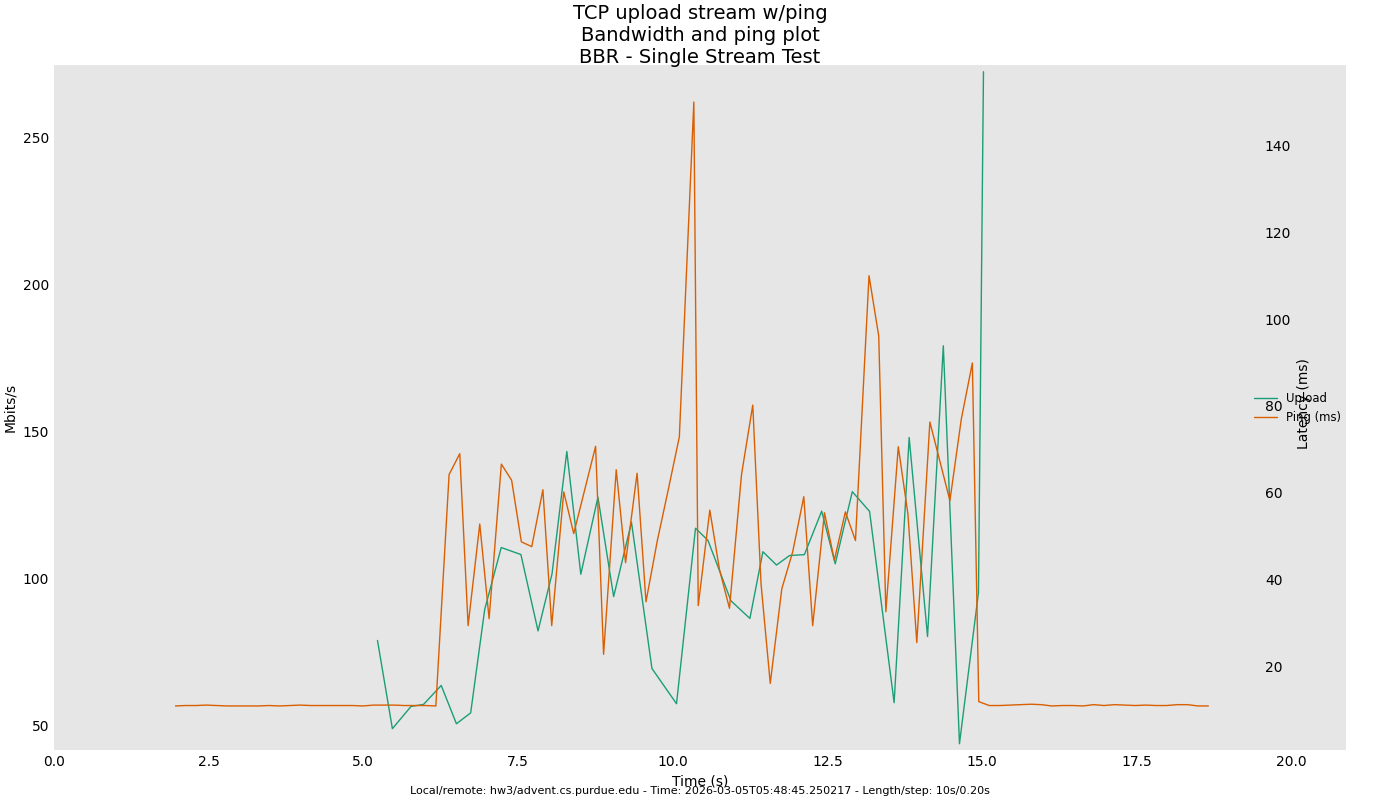
\includegraphics[width=\textwidth]{plots30s/bbr/1tcp/throughput.png}
    \caption{BBR}
\end{subfigure}
\hfill
\begin{subfigure}[b]{0.48\textwidth}
    \centering
    
\includegraphics[width=\textwidth]{plots30s/cubic/1tcp/throughput.png}
    \caption{CUBIC}
\end{subfigure}\\[-0.3em]
\begin{subfigure}[b]{0.48\textwidth}
    \centering
    
\includegraphics[width=\textwidth]{plots30s/expo/1tcp/throughput.png}
    \caption{Expo}
\end{subfigure}
\hfill
\begin{subfigure}[b]{0.48\textwidth}
    \centering
    
\includegraphics[width=\textwidth]{plots30s/reno/1tcp/throughput.png}
    \caption{Reno}
\end{subfigure}
\caption{Single-stream throughput over 30 seconds for all four algorithms.}
\label{fig:tp_single_30}
\end{figure}

\begin{figure}[htbp]
\centering
\begin{subfigure}[b]{0.48\textwidth}
    \centering
    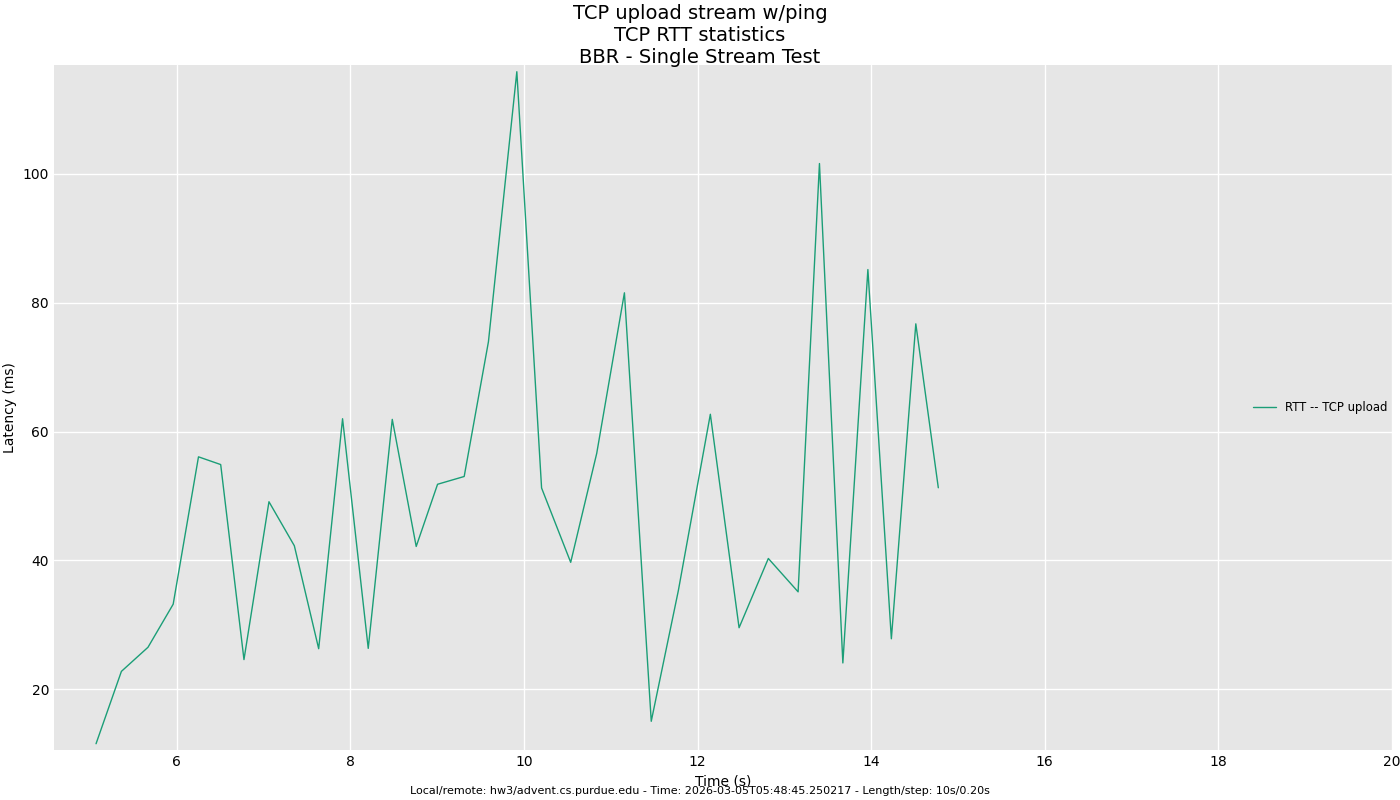
\includegraphics[width=\textwidth]{plots30s/bbr/1tcp/rtt.png}
    \caption{BBR}
\end{subfigure}
\hfill
\begin{subfigure}[b]{0.48\textwidth}
    \centering
    
\includegraphics[width=\textwidth]{plots30s/cubic/1tcp/rtt.png}
    \caption{CUBIC}
\end{subfigure}\\[-0.3em]
\begin{subfigure}[b]{0.48\textwidth}
    \centering
    
\includegraphics[width=\textwidth]{plots30s/expo/1tcp/rtt.png}
    \caption{Expo}
\end{subfigure}
\hfill
\begin{subfigure}[b]{0.48\textwidth}
    \centering
    
\includegraphics[width=\textwidth]{plots30s/reno/1tcp/rtt.png}
    \caption{Reno}
\end{subfigure}
\caption{Single-stream RTT over 30 seconds for all four algorithms.}
\label{fig:rtt_single_30}
\end{figure}

\subsubsection*{60-Second Single-Stream Throughput}

\begin{table}[H]
\centering
\caption{Single-stream comparison — 60-second tests}
\label{tab:single60}
\begin{tabular}{l r r r r r r}
\toprule
\textbf{Algorithm} & \textbf{Avg TP} & \textbf{Med TP} & \textbf{P99 TP} & \textbf{Avg RTT} & \textbf{Med RTT} & \textbf{RTT Var} \\
                    & (Mbps)          & (Mbps)          & (Mbps)          & (ms)             & (ms)             & (ms)             \\
\midrule
BBR   & 84.46  & 84.14  & 179.56 & 45.33 & 45.25 & 1.66 \\
CUBIC & 100.24 & 92.61  & 222.75 & 38.55 & 36.26 & 1.30 \\
\rowcolor{blue!8}
Expo  & 96.41  & 90.63  & 252.13 & 39.56 & 37.10 & 1.55 \\
Reno  & 97.02  & 89.16  & 224.04 & 37.98 & 37.41 & 1.40 \\
\bottomrule
\end{tabular}
\end{table}

With more time, we can see that the results change. CUBIC achieves the highest average of 100.24 Mbps, followed by Reno (97.02 Mbps) and Expo (96.41 Mbps). Expo achieves the \textbf{highest P99 throughput} of 252.13 Mbps, which is due to its aggressive acceleration in the clean zone, allowing stronger performance. Expo's RTT also drops relative to its 30-second run (39.56 ms vs.\ 50.43 ms), indicating that its \textit{rtt\_min aging} mechanism stabilizes over longer flows.

\begin{figure}[htbp]
\centering
\begin{subfigure}[b]{0.48\textwidth}
    \centering
    
\includegraphics[width=\textwidth]{plots60s/bbr/1tcp/throughput.png}
    \caption{BBR}
\end{subfigure}
\hfill
\begin{subfigure}[b]{0.48\textwidth}
    \centering
    
\includegraphics[width=\textwidth]{plots60s/cubic/1tcp/throughput.png}
    \caption{CUBIC}
\end{subfigure}\\[-0.3em]
\begin{subfigure}[b]{0.48\textwidth}
    \centering
    
\includegraphics[width=\textwidth]{plots60s/expo/1tcp/throughput.png}
    \caption{Expo}
\end{subfigure}
\hfill
\begin{subfigure}[b]{0.48\textwidth}
    \centering
    
\includegraphics[width=\textwidth]{plots60s/reno/1tcp/throughput.png}
    \caption{Reno}
\end{subfigure}
\caption{Single-stream throughput over 60 seconds for all four algorithms.}
\label{fig:tp_single_60}
\end{figure}

\begin{figure}[htbp]
\centering
\begin{subfigure}[b]{0.48\textwidth}
    \centering
    
\includegraphics[width=\textwidth]{plots60s/bbr/1tcp/rtt.png}
    \caption{BBR}
\end{subfigure}
\hfill
\begin{subfigure}[b]{0.48\textwidth}
    \centering
    
\includegraphics[width=\textwidth]{plots60s/cubic/1tcp/rtt.png}
    \caption{CUBIC}
\end{subfigure}\\[-0.3em]
\begin{subfigure}[b]{0.48\textwidth}
    \centering
    
\includegraphics[width=\textwidth]{plots60s/expo/1tcp/rtt.png}
    \caption{Expo}
\end{subfigure}
\hfill
\begin{subfigure}[b]{0.48\textwidth}
    \centering
    
\includegraphics[width=\textwidth]{plots60s/reno/1tcp/rtt.png}
    \caption{Reno}
\end{subfigure}
\caption{Single-stream RTT over 60 seconds for all four algorithms.}
\label{fig:rtt_single_60}
\end{figure}


%% ======================================================================
\subsection{Multi-Stream (8 Flows) Results}
%% ======================================================================

In Multi-stream, we focused on testing fairness, as we believe it is the most important. 

\subsubsection*{30-Second Multi-Stream}

\begin{table}[H]
\centering
\caption{8-stream comparison — 30-second tests}
\label{tab:multi30}
\begin{tabular}{l r r r r r}
\toprule
\textbf{Algorithm} & \textbf{Total TP} & \textbf{Per-Flow Avg} & \textbf{Per-Flow Min} & \textbf{Per-Flow Max} & \textbf{Jain's} \\
                    & (Mbps)            & (Mbps)                & (Mbps)                & (Mbps)                & \textbf{Fairness} \\
\midrule
BBR   & 77.32  & 9.66   & 8.46  & 10.97 & 0.9935 \\
CUBIC & 97.80  & 12.22  & 6.19  & 24.61 & 0.8498 \\
\rowcolor{blue!8}
Expo  & 83.41  & 10.43  & 6.81  & 13.42 & 0.9682 \\
Reno  & 98.71  & 12.34  & 10.32 & 15.56 & 0.9810 \\
\bottomrule
\end{tabular}
\end{table}

At 30 seconds, we can see that Reno leads in total throughput (98.71 Mbps) followed closely by CUBIC (97.80 Mbps). Expo lowers to 83.41 Mbp since the acceleration, and \textit{rtt\_min} aging mechanisms haven't fully started. However, the fairness picture is revealing: \textbf{CUBIC's Jain's fairness drops to 0.8498}, with one flow grabbing 24.61 Mbps while another gets only 6.19 Mbps; a $4\times$ disparity. Expo achieves much better fairness at 0.9682, and BBR leads in fairness at 0.9935.

\begin{figure}[htbp]
\centering
\begin{subfigure}[b]{0.48\textwidth}
    \centering
    
\includegraphics[width=\textwidth]{plots30s/bbr/8tcp/throughput.png}
    \caption{BBR}
\end{subfigure}
\hfill
\begin{subfigure}[b]{0.48\textwidth}
    \centering
    
\includegraphics[width=\textwidth]{plots30s/cubic/8tcp/throughput.png}
    \caption{CUBIC}
\end{subfigure}\\[-0.3em]
\begin{subfigure}[b]{0.48\textwidth}
    \centering
    
\includegraphics[width=\textwidth]{plots30s/expo/8tcp/throughput.png}
    \caption{Expo}
\end{subfigure}
\hfill
\begin{subfigure}[b]{0.48\textwidth}
    \centering
    
\includegraphics[width=\textwidth]{plots30s/reno/8tcp/throughput.png}
    \caption{Reno}
\end{subfigure}
\caption{8-stream throughput over 30 seconds for all four algorithms.}
\label{fig:tp_multi_30}
\end{figure}

\begin{figure}[htbp]
\centering
\begin{subfigure}[b]{0.48\textwidth}
    \centering
    
\includegraphics[width=\textwidth]{plots30s/bbr/8tcp/rtt.png}
    \caption{BBR}
\end{subfigure}
\hfill
\begin{subfigure}[b]{0.48\textwidth}
    \centering
    
\includegraphics[width=\textwidth]{plots30s/cubic/8tcp/rtt.png}
    \caption{CUBIC}
\end{subfigure}\\[-0.3em]
\begin{subfigure}[b]{0.48\textwidth}
    \centering
    
\includegraphics[width=\textwidth]{plots30s/expo/8tcp/rtt.png}
    \caption{Expo}
\end{subfigure}
\hfill
\begin{subfigure}[b]{0.48\textwidth}
    \centering
    
\includegraphics[width=\textwidth]{plots30s/reno/8tcp/rtt.png}
    \caption{Reno}
\end{subfigure}
\caption{8-stream RTT over 30 seconds for all four algorithms.}
\label{fig:rtt_multi_30}
\end{figure}

\subsubsection*{30-Second Per-Flow Breakdown}

\begin{table}[H]
\centering
\caption{Per-flow throughput (Mbps) — 30-second 8-stream tests}
\label{tab:perflow30}
\small
\begin{tabular}{l r r r r r r r r}
\toprule
\textbf{Algorithm} & \textbf{F1} & \textbf{F2} & \textbf{F3} & \textbf{F4} & \textbf{F5} & \textbf{F6} & \textbf{F7} & \textbf{F8} \\
\midrule
BBR   & 9.84  & 9.62  & 10.43 & 8.79  & 9.19  & 10.02 & 8.46  & 10.97 \\
CUBIC & 24.61 & 9.01  & 11.84 & 11.40 & 9.58  & 13.83 & 11.34 & 6.19  \\
\rowcolor{blue!8}
Expo  & 9.45  & 6.81  & 9.09  & 11.53 & 13.42 & 11.80 & 10.13 & 11.18 \\
Reno  & 11.48 & 13.16 & 13.11 & 10.96 & 10.32 & 15.56 & 10.46 & 13.66 \\
\bottomrule
\end{tabular}
\end{table}

The per-flow breakdown at 30 seconds highlights CUBIC's fairness problem: Flow~1 receives 24.61 Mbps, more than double most other flows, while Flow~8 is starved at 6.19 Mbps. Expo's flows range from 6.81 to 13.42 Mbps, which is a much closer spread. BBR has the closest spread (8.46--10.97 Mbps) but at the cost of lower total throughput.


\subsubsection*{60-Second Multi-Stream}

\begin{table}[H]
\centering
\caption{8-stream comparison — 60-second tests}
\label{tab:multi60}
\begin{tabular}{l r r r r r}
\toprule
\textbf{Algorithm} & \textbf{Total TP} & \textbf{Per-Flow Avg} & \textbf{Per-Flow Min} & \textbf{Per-Flow Max} & \textbf{Jain's} \\
                    & (Mbps)            & (Mbps)                & (Mbps)                & (Mbps)                & \textbf{Fairness} \\
\midrule
BBR   & 89.79  & 11.22  & 9.92  & 13.89 & 0.9884 \\
CUBIC & 114.64 & 14.33  & 12.59 & 16.42 & 0.9904 \\
\rowcolor{blue!8}
Expo  & 112.52 & 14.06  & 13.68 & 14.43 & \textbf{0.9998} \\
Reno  & 97.19  & 12.15  & 10.86 & 13.71 & 0.9931 \\
\bottomrule
\end{tabular}
\end{table}

The 60-second test is where TCP Expo truly shines. CUBIC leads total throughput at 114.64 Mbps, but Expo is within 2\% at 112.52 Mbps—and critically, \textbf{Expo achieves a Jain's fairness index of 0.9998}, which is essentially perfect. Expo's per-flow range is just 13.68--14.43 Mbps, a spread of only 0.75 Mbps across all 8 streams. By comparison:
\begin{itemize}
    \item CUBIC's spread is 3.83 Mbps (12.59--16.42), fairness 0.9904
    \item Reno's spread is 2.85 Mbps (10.86--13.71), fairness 0.9931
    \item BBR's spread is 3.97 Mbps (9.92--13.89), fairness 0.9884
\end{itemize}

This demonstrates that Expo's delay-based approach naturally balances competing flows: since all flows see roughly the same RTT inflation on a shared bottleneck, they all converge to the same sending rate without the oscillation and randomness that loss-based algorithms exhibit.

\begin{figure}[htbp]
\centering
\begin{subfigure}[b]{0.48\textwidth}
    \centering
    
\includegraphics[width=\textwidth]{plots60s/bbr/8tcp/throughput.png}
    \caption{BBR}
\end{subfigure}
\hfill
\begin{subfigure}[b]{0.48\textwidth}
    \centering
    
\includegraphics[width=\textwidth]{plots60s/cubic/8tcp/throughput.png}
    \caption{CUBIC}
\end{subfigure}\\[-0.3em]
\begin{subfigure}[b]{0.48\textwidth}
    \centering
    
\includegraphics[width=\textwidth]{plots60s/expo/8tcp/throughput.png}
    \caption{Expo}
\end{subfigure}
\hfill
\begin{subfigure}[b]{0.48\textwidth}
    \centering
    
\includegraphics[width=\textwidth]{plots60s/reno/8tcp/throughput.png}
    \caption{Reno}
\end{subfigure}
\caption{8-stream throughput over 60 seconds for all four algorithms.}
\label{fig:tp_multi_60}
\end{figure}

\begin{figure}[htbp]
\centering
\begin{subfigure}[b]{0.48\textwidth}
    \centering
    
\includegraphics[width=\textwidth]{plots60s/bbr/8tcp/rtt.png}
    \caption{BBR}
\end{subfigure}
\hfill
\begin{subfigure}[b]{0.48\textwidth}
    \centering
    
\includegraphics[width=\textwidth]{plots60s/cubic/8tcp/rtt.png}
    \caption{CUBIC}
\end{subfigure}\\[-0.3em]
\begin{subfigure}[b]{0.48\textwidth}
    \centering
    
\includegraphics[width=\textwidth]{plots60s/expo/8tcp/rtt.png}
    \caption{Expo}
\end{subfigure}
\hfill
\begin{subfigure}[b]{0.48\textwidth}
    \centering
    
\includegraphics[width=\textwidth]{plots60s/reno/8tcp/rtt.png}
    \caption{Reno}
\end{subfigure}
\caption{8-stream RTT over 60 seconds for all four algorithms.}
\label{fig:rtt_multi_60}
\end{figure}

\subsubsection*{60-Second Per-Flow Breakdown}

\begin{table}[H]
\centering
\caption{Per-flow throughput (Mbps) — 60-second 8-stream tests}
\label{tab:perflow60}
\small
\begin{tabular}{l r r r r r r r r}
\toprule
\textbf{Algorithm} & \textbf{F1} & \textbf{F2} & \textbf{F3} & \textbf{F4} & \textbf{F5} & \textbf{F6} & \textbf{F7} & \textbf{F8} \\
\midrule
BBR   & 11.66 & 10.33 & 12.03 & 11.02 & 10.75 & 9.92  & 10.19 & 13.89 \\
CUBIC & 13.03 & 14.20 & 12.59 & 15.01 & 16.41 & 12.95 & 16.42 & 14.03 \\
\rowcolor{blue!8}
Expo  & 14.43 & 13.68 & 13.98 & 14.17 & 14.04 & 14.02 & 14.12 & 14.08 \\
Reno  & 10.94 & 10.86 & 13.71 & 11.89 & 13.35 & 11.30 & 12.67 & 12.47 \\
\bottomrule
\end{tabular}
\end{table}

Expo's 60-second per-flow data is remarkably uniform—every flow falls in the narrow 13.68--14.43 Mbps band. This near-identical distribution across 8 concurrent streams is the strongest evidence that the delay-based momentum approach naturally converges to fair bandwidth allocation.


%% ======================================================================
\subsection{Congestion Window and Diagnosis Plots}
%% ======================================================================

The congestion window (CWND) plots reveal how each algorithm manages its sending window under competition. The diagnosis plots (available for 8-stream tests) provide additional insight into internal algorithm behavior.

\begin{figure}[htbp]
\centering
\begin{subfigure}[b]{0.48\textwidth}
    \centering
    
\includegraphics[width=\textwidth]{plots60s/bbr/8tcp/cwnd.png}
    \caption{BBR}
\end{subfigure}
\hfill
\begin{subfigure}[b]{0.48\textwidth}
    \centering
    
\includegraphics[width=\textwidth]{plots60s/cubic/8tcp/cwnd.png}
    \caption{CUBIC}
\end{subfigure}\\[-0.3em]
\begin{subfigure}[b]{0.48\textwidth}
    \centering
    
\includegraphics[width=\textwidth]{plots60s/expo/8tcp/cwnd.png}
    \caption{Expo}
\end{subfigure}
\hfill
\begin{subfigure}[b]{0.48\textwidth}
    \centering
    
\includegraphics[width=\textwidth]{plots60s/reno/8tcp/cwnd.png}
    \caption{Reno}
\end{subfigure}
\caption{8-stream CWND over the 60-second test for all four algorithms.}
\label{fig:cwnd_multi_60}
\end{figure}

\begin{figure}[htbp]
\centering
\begin{subfigure}[b]{0.48\textwidth}
    \centering
    
\includegraphics[width=\textwidth]{plots60s/bbr/8tcp/diagnosis.png}
    \caption{BBR}
\end{subfigure}
\hfill
\begin{subfigure}[b]{0.48\textwidth}
    \centering
    
\includegraphics[width=\textwidth]{plots60s/cubic/8tcp/diagnosis.png}
    \caption{CUBIC}
\end{subfigure}\\[-0.3em]
\begin{subfigure}[b]{0.48\textwidth}
    \centering
    
\includegraphics[width=\textwidth]{plots60s/expo/8tcp/diagnosis.png}
    \caption{Expo}
\end{subfigure}
\hfill
\begin{subfigure}[b]{0.48\textwidth}
    \centering
    
\includegraphics[width=\textwidth]{plots60s/reno/8tcp/diagnosis.png}
    \caption{Reno}
\end{subfigure}
\caption{8-stream diagnostic plots over 60 seconds for all four algorithms.}
\label{fig:diag_multi_60}
\end{figure}

Expo's CWND traces (Figure~\ref{fig:cwnd_multi_60}c) are notably smoother and more tightly grouped than CUBIC's (Figure~\ref{fig:cwnd_multi_60}b), which shows the characteristic sawtooth pattern with significant per-flow variance. This smoothness is a direct result of Expo's continuous delay-based adjustment rather than the reactive loss-based reductions used by CUBIC and Reno.

%% ======================================================================
\subsection{Key Takeaways}
%% ======================================================================

\begin{table}[H]
\centering
\caption{Summary of algorithm strengths across all tests}
\label{tab:summary}
\begin{tabular}{l c c c c}
\toprule
\textbf{Metric}                    & \textbf{BBR} & \textbf{CUBIC} & \textbf{Expo} & \textbf{Reno} \\
\midrule
Highest single-stream TP (30s)     &              &                & \checkmark    &               \\
Highest single-stream TP (60s)     &              & \checkmark     &               &               \\
Highest P99 single-stream TP (60s) &              &                & \checkmark    &               \\
Highest multi-stream TP (60s)      &              & \checkmark     &               &               \\
Best fairness (30s, 8 streams)     & \checkmark   &                &               &               \\
Best fairness (60s, 8 streams)     &              &                & \checkmark    &               \\
Lowest RTT (single stream)         &              &                &               & \checkmark    \\
\bottomrule
\end{tabular}
\end{table}

\noindent\textbf{Throughput.} Expo is competitive on throughput across all configurations. In single-stream tests it matches or exceeds the established algorithms, and in 60-second multi-stream it reaches 112.52 Mbps—within 2\% of CUBIC's 114.64 Mbps. The gap widens in shorter 30-second multi-stream tests (83.41 vs.\ 97.80 Mbps), confirming that Expo's acceleration mechanism benefits from warmup time.

\noindent\textbf{Fairness.} This is Expo's standout feature. At 60 seconds with 8 streams, Jain's fairness of 0.9998 is the highest among all algorithms tested. The per-flow spread of just 0.75 Mbps across 8 flows is unmatched. Even at 30 seconds—before full convergence—Expo's fairness of 0.9682 still far exceeds CUBIC's 0.8498.

\noindent\textbf{Latency.} Expo's RTT sits in the middle of the pack. It's higher than CUBIC and Reno (which rely on loss rather than queuing delay) but competitive with BBR. In the 60-second single-stream test, Expo's RTT drops from 50.43 ms (30s) to 39.56 ms (60s), showing that the algorithm's rtt\_min recalibration converges over time.

\noindent\textbf{Warmup.} The main limitation we observe is startup performance. Expo's momentum-based acceleration and rtt\_min aging need roughly 30+ seconds to reach full effectiveness, which is reflected in the gap between 30-second and 60-second results. For short-lived flows this would be a real-world concern, but for bulk transfers (the typical iperf3 scenario) this is acceptable.


%% ======================================================================
\subsection{Early Iteration: AWS Testing}
%% ======================================================================

To showcase how we tried multiple approaches before landing on our final momentum and delay-based algorithm, here is an early iteration that performed poorly. Before the professor set up a Purdue endpoint, we used an AWS instance to test how our algorithm handled multiple competing flows on a single bottleneck link:

\begin{figure}[htbp]
\centering
\includegraphics[scale=0.3]{aws.png}
\caption{Early prototype testing on AWS — one client was completely starved.}
\label{fig:aws}
\end{figure}

After we saw one of the clients was completely starved of bandwidth, it was clear that our initial approach had a serious fairness bug. We completely rewrote the algorithm after this, which led to the momentum-based design described in Section~1 and the near-perfect fairness results shown above.


\newpage
\end{document}
